\documentclass{article}[18pt]
\ProvidesPackage{format}
%Page setup
\usepackage[utf8]{inputenc}
\usepackage[margin=0.7in]{geometry}
\usepackage{parselines} 
\usepackage[english]{babel}
\usepackage{fancyhdr}
\usepackage{titlesec}
\hyphenpenalty=10000

\pagestyle{fancy}
\fancyhf{}
\rhead{Sam Robbins}
\rfoot{Page \thepage}

%Characters
\usepackage{amsmath}
\usepackage{amssymb}
\usepackage{gensymb}
\newcommand{\R}{\mathbb{R}}

%Diagrams
\usepackage{pgfplots}
\usepackage{graphicx}
\usepackage{tabularx}
\usepackage{relsize}
\pgfplotsset{width=10cm,compat=1.9}
\usepackage{float}

%Length Setting
\titlespacing\section{0pt}{14pt plus 4pt minus 2pt}{0pt plus 2pt minus 2pt}
\newlength\tindent
\setlength{\tindent}{\parindent}
\setlength{\parindent}{0pt}
\renewcommand{\indent}{\hspace*{\tindent}}

%Programming Font
\usepackage{courier}
\usepackage{listings}
\usepackage{pxfonts}

%Lists
\usepackage{enumerate}
\usepackage{enumitem}

% Networks Macro
\usepackage{tikz}


% Commands for files converted using pandoc
\providecommand{\tightlist}{%
	\setlength{\itemsep}{0pt}\setlength{\parskip}{0pt}}
\usepackage{hyperref}

% Get nice commands for floor and ceil
\usepackage{mathtools}
\DeclarePairedDelimiter{\ceil}{\lceil}{\rceil}
\DeclarePairedDelimiter{\floor}{\lfloor}{\rfloor}

% Allow itemize to go up to 20 levels deep (just change the number if you need more you madman)
\usepackage{enumitem}
\setlistdepth{20}
\renewlist{itemize}{itemize}{20}

% initially, use dots for all levels
\setlist[itemize]{label=$\cdot$}

% customize the first 3 levels
\setlist[itemize,1]{label=\textbullet}
\setlist[itemize,2]{label=--}
\setlist[itemize,3]{label=*}

% Definition and Important Stuff
% Important stuff
\usepackage[framemethod=TikZ]{mdframed}

\newcounter{theo}[section]\setcounter{theo}{0}
\renewcommand{\thetheo}{\arabic{section}.\arabic{theo}}
\newenvironment{important}[1][]{%
	\refstepcounter{theo}%
	\ifstrempty{#1}%
	{\mdfsetup{%
			frametitle={%
				\tikz[baseline=(current bounding box.east),outer sep=0pt]
				\node[anchor=east,rectangle,fill=red!50]
				{\strut Important};}}
	}%
	{\mdfsetup{%
			frametitle={%
				\tikz[baseline=(current bounding box.east),outer sep=0pt]
				\node[anchor=east,rectangle,fill=red!50]
				{\strut Important:~#1};}}%
	}%
	\mdfsetup{innertopmargin=10pt,linecolor=red!50,%
		linewidth=2pt,topline=true,%
		frametitleaboveskip=\dimexpr-\ht\strutbox\relax
	}
	\begin{mdframed}[]\relax%
		\centering
		}{\end{mdframed}}



\newcounter{lem}[section]\setcounter{lem}{0}
\renewcommand{\thelem}{\arabic{section}.\arabic{lem}}
\newenvironment{defin}[1][]{%
	\refstepcounter{lem}%
	\ifstrempty{#1}%
	{\mdfsetup{%
			frametitle={%
				\tikz[baseline=(current bounding box.east),outer sep=0pt]
				\node[anchor=east,rectangle,fill=blue!20]
				{\strut Definition};}}
	}%
	{\mdfsetup{%
			frametitle={%
				\tikz[baseline=(current bounding box.east),outer sep=0pt]
				\node[anchor=east,rectangle,fill=blue!20]
				{\strut Definition:~#1};}}%
	}%
	\mdfsetup{innertopmargin=10pt,linecolor=blue!20,%
		linewidth=2pt,topline=true,%
		frametitleaboveskip=\dimexpr-\ht\strutbox\relax
	}
	\begin{mdframed}[]\relax%
		\centering
		}{\end{mdframed}}
\lhead{Software Engineering - Software Development}


\begin{document}
\begin{center}
\underline{\huge SDLC and Standards}
\end{center}
\section{Software Development Lifecycle}
\begin{center}
	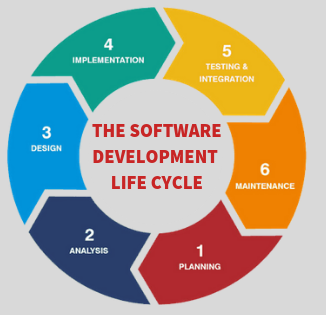
\includegraphics[scale=0.7]{Lifecycle}
\end{center}
\begin{itemize}
	\item The SDLC framework is used in industry to design, develop and test high quality software
	\item Focussing on creating software that meets the needs and expectations of the client
	\item Within the client's timeline and budget
\end{itemize}
\section{Phases}
\subsection{Planning and RE(requirements) analysis}
\begin{itemize}
	\item Planning is the first and most fundamental of the phases
	\item Get this wrong and nothing else will work
	\item Inc. quality assurance and risk analysis
\end{itemize}
Stakeholders/Roles within this phase
\begin{itemize}
	\item Client
	\item Customer
	\item Approver (managerial oversight)
	\item Assessor (some degree of technical expertise to advise)
\end{itemize}
Outcome
\begin{itemize}
	\item An approved proposal
	\item A functional requirements doc
\end{itemize}
\subsection{Design}
\begin{itemize}
	\item The goal here is to create the s/w design document(s) based on the inputs from the previous phase (planning and analysis)
	\item Perform design discussions, examine design patterns, consider requirements
	\item Output: systems design docs for DB, API, application, infrastructure, testing, training, maintenance, user ...
\end{itemize}
Roles:
\begin{itemize}
	\item \textbf{End user} - final users of system
	\item \textbf{Business analyst} - provide requirements to the design team, review solution design and artefacts
	\item \textbf{Project Manager} - Finalize data conversion strategy and test strategy, review solution design and artefacts
	\item \textbf{Technical-Architect, Tech-Designer, Design-Team} - Design system architecture, software components, etc; design walk-through
	\item \textbf{Developer/Construction Team} - Assist with identifying and finalizing testing strategy; review of the architecture and software components
	\item \textbf{Database team} - Assist with architecture design and data conversion strategy
\end{itemize}
\subsection{Implementation}
\begin{itemize}
	\item Get your hands dirty with coding
	\item Your teams may use any approach that works for you
	\item Within a business you will have to abide by their coding guidelines
\end{itemize}
Roles:
\begin{itemize}
	\item \textbf{Customer}, sponsor and signs off team effort; review progress with the developers and the PM.
	\item \textbf{Project Manager}, resolve resource, scheduling, budget issues; review and report progress.
	\item \textbf{Developer}, construct a working solution from the approved design; produce artifacts and put them under configuration control and perform change control; employ tools, systems and conform to prescribed standards (platforms, coding practices, programming languages, etc) that are in line with the organization’s objectives.
	\item \textbf{Database Administration Group}, assist with implementing the solution design and data conversion strategy.
	\item \textbf{Implementation supervisor/manager}, assist with identifying the requirements for implementation of the solution (which includes system readiness, resources, time-lines).
	\item \textbf{Integration supervisor/manager}, identify how integration of the solution in a new hardware/software  environment would be achieved; what tests are required to evaluate integration.
\end{itemize}
\subsection{Testing \& Integration/Deployment}
\begin{itemize}
	\item These phases are sometimes separated
	\item The goal of testing is to check that the development is functional and meets requirements
	\item Complexity arises from integration of a novel system with existing (sub-)systems
	\item Test for various functional attributes
	\begin{itemize}
		\item Security, conformance, accessibility, performance, stress
	\end{itemize}
\end{itemize}
Roles:
\begin{itemize}
	\item \textbf{Project Manager}, resolve resource, scheduling, budget issues; review and report progress.
	\item \textbf{Developer}, assist with building tests and analysis of test results.
	\item \textbf{Database Administration Group}, assist with integration of the solution design and data conversion tests.
	\item \textbf{Implementation manager}, assist with analysis of test results.
	\item \textbf{Integration manager}, assist with analysis of test results.
\end{itemize}
Sign off is completed when the functional requirements specification has been met
\subsection{Implementation}
\begin{itemize}
	\item Some versions of the SDLC have an additional phase here
	\item The focus is to install the system in the production environment and to bring it into \textbf{operation}; and then to ensure that the system:
	\begin{itemize}
		\item Satisfies the functional requirements
		\item Satisfies the business needs
		\item Adheres to all mandates, physical constraints and service level agreements
		\item Operates as described in the User and Operator Manuals
	\end{itemize}
\end{itemize}
\subsection{Maintenance}
\begin{itemize}
	\item On successful operational transfer of the project, development group hands over to the maintenance group
	\item Documentation must be ready for transfer at this time
	\item Roles:
	\begin{itemize}
		\item \textbf{Solution Delivery Team} – Prepares all solution documentation 
		and manuals for the maintenance group.  The solution delivery 
		team will supply any requested training to help maintenance 
		team technicians learn the solution’s behaviours
		\item \textbf{Solution Maintenance Team} – Reviews all solution 
		documentation and supports the solution until the terms 
		of the maintenance agreement expire
	\end{itemize}
\end{itemize}
\section{Alternatives}
There are many correct models depending on the people and project. The SDLC just outlines the phases
\section{Standards}


\end{document}